\documentclass{article}
\usepackage{amsmath,amsthm,amssymb,amsfonts}
\usepackage{setspace,enumitem}
\usepackage{graphicx}
\usepackage{hyperref}
\usepackage{natbib}
\usepackage{lscape}
\usepackage{afterpage}
\usepackage{xcolor}
\usepackage{etoolbox}
\usepackage{booktabs}
\usepackage{pdfpages}
\usepackage{multicol}
\usepackage{geometry}
\usepackage{accents}
\usepackage{bbm}
\hypersetup{
	colorlinks,
	linkcolor={blue!90!black},
	citecolor={red!90!black},
	urlcolor={blue!90!black}
}

\newtheorem{theorem}{Theorem}
\newtheorem{assumption}{Assumption}
\newtheorem{definition}{Definition}
\newtheorem{lemma}{Lemma}
\setlength{\parindent}{0cm}
\geometry{margin = 1in}

\newcommand{\R}{\mathbb{R}}
\newcommand{\ubar}[1]{\underaccent{\bar}{#1}}
\newcommand{\Int}{\text{Int}}
\newcommand{\xbf}{\mathbf{x}}
\newcommand{\Abf}{\mathbf{A}}
\newcommand{\Bbf}{\mathbf{B}}
\newcommand{\Gbf}{\mathbf{G}}
\newcommand{\bbf}{\mathbf{b}}
\newcommand{\one}{\mathbbm{1}}

\newtoggle{extended}
\settoggle{extended}{false}

\title{FIN 971A: Homework 1}
\author{Alex von Hafften }

\begin{document}

\maketitle

\section{Question 1}

Below is my replication of table 1 from LRZ (2008) for all firms.  The numbers line up relatively well with LRZ.  My method of filtering the data resulted in a smaller dataset by half.  I tried my best to follow their description in the beginning of section 1.  I limited the sample to observations with reported book assets and book and market leverage between zero and one.  Furthermore, I computed the 1st and 99th percentile for each variable and then drop observations that fell outside of that for one of the variables. The statistics for book leverage, market leverage, log sales, market-to-book, tangibility, median industry book leverage, and intangible assets are pretty close.  My statistics for profitability and cash flow volatility are about half of LRZ.  One contributing factor could have been that I scaled both cash flow volatility and intangible assets by book assets (the data appendix is silent on any scaling); otherwise they would be in dollar terms.  Another omission from the data appendix is the definition of dividend payer.  Here, I pull Compustat variable \texttt{dv}, which is the cash dividend, and defined ``Dividend Payer" as a dummy that equals one if \texttt{dv} is greater than zero.

\bigskip

{
\def\sym#1{\ifmmode^{#1}\else\(^{#1}\)\fi}
\begin{tabular}{l*{1}{cccc}}
\hline\hline
                    &        Mean&      Median&          SD&           N\\
\hline
Book\_Leverage       &        0.25&        0.24&        0.19&     108,166\\
Market\_Leverage     &        0.30&        0.25&        0.25&     108,166\\
log\_Sales           &        4.73&        4.69&        2.05&     108,166\\
Market\_to\_Book      &        1.26&        0.91&        1.12&     108,166\\
Profitability       &        0.10&        0.12&        0.15&     108,166\\
Tangibility         &        0.33&        0.28&        0.24&     108,166\\
Cash\_Flow\_Volatility&        0.05&        0.03&        0.06&     108,166\\
Median\_Industry\_Book\_Leverage&        0.23&        0.24&        0.10&     108,166\\
Dividend\_Payer      &        0.55&        1.00&        0.50&     108,166\\
Intangible\_Assets   &        0.06&        0.01&        0.10&     108,166\\
\hline\hline
\end{tabular}
}


\bigskip

Below is my replication of table 1 from LRZ (2008) for survivor firms. Similar to all firms, my sample is about half that of LRZ (2008). The same statistics as above (plus profitability) are close to that of LRZ, but my statistics for cash flow volatility are similarly about half of LRZ.

\bigskip

{
\def\sym#1{\ifmmode^{#1}\else\(^{#1}\)\fi}
\begin{tabular}{l*{1}{cccc}}
\hline\hline
                    &        Mean&      Median&          SD&           N\\
\hline
Book\_Leverage       &        0.26&        0.25&        0.17&      49,950\\
Market\_Leverage     &        0.31&        0.27&        0.24&      49,950\\
log\_Sales           &        5.34&        5.34&        1.99&      49,950\\
Market\_to\_Book      &        1.14&        0.86&        0.90&      49,950\\
Profitability       &        0.13&        0.13&        0.10&      49,950\\
Tangibility         &        0.36&        0.31&        0.23&      49,950\\
Cash\_Flow\_Volatility&        0.04&        0.03&        0.04&      49,950\\
Median\_Industry\_Book\_Leverage&        0.25&        0.25&        0.09&      49,950\\
Dividend\_Payer      &        0.73&        1.00&        0.45&      49,950\\
Intangible\_Assets   &        0.04&        0.00&        0.08&      49,950\\
\hline\hline
\end{tabular}
}


\pagebreak

\begin{landscape}
\section{Question 2}

Below is my replication of panel A (all firms) of table 2 in LRZ (2008). As in LRZ, I normalized all independent variables (i.e. minus mean divided by standard deviation), so the coefficient is the change in the leverage ratio in pp given a one standard deviation change in the independent variable.

\begin{enumerate}

\item My coefficient estimate is much lower than LRZ as well as a much lower R-squared. This finding would contest their argument that initial leverage is such as important determinant of future leverage.

\item My coefficient estimates are much closer to LRZ. For example, same significant variables with the same sign.

\item Similar to (2). I do get a negative coefficent on cash flow volatility unlike LRZ.

\item Similar finding to (1). Much lower coefficient and lower R-squared.

\item Similar to (2). Coefficients are closer to LRZ in terms of significance and sign.

\item Same as (3).

\end{enumerate}

\bigskip

\begin{tabular}{lcccccc} \hline
 & (1) & (2) & (3) & (4) & (5) & (6) \\
VARIABLES & b\_lev\_tr & b\_lev\_tr & b\_lev\_tr & m\_lev\_tr & m\_lev\_tr & m\_lev\_tr \\ \hline
 &  &  &  &  &  &  \\
zee\_i\_b\_lev & 0.0274 & 0.0227 & 0.0180 &  &  &  \\
 & (0.0242) & (0.0198) & (0.0167) &  &  &  \\
zee\_l\_sales\_tr &  & 0.0189*** & 0.0257*** &  & 0.0248*** & 0.0351*** \\
 &  & (0.00166) & (0.00175) &  & (0.00175) & (0.00184) \\
zee\_m\_b\_tr &  & -0.0304*** & -0.0174*** &  & -0.0830*** & -0.0743*** \\
 &  & (0.00149) & (0.00130) &  & (0.00155) & (0.00148) \\
zee\_profit\_tr &  & -0.0341*** & -0.0396*** &  & -0.0536*** & -0.0596*** \\
 &  & (0.00135) & (0.00134) &  & (0.00142) & (0.00140) \\
zee\_tang\_tr &  & 0.0525*** & 0.0314*** &  & 0.0353*** & 0.0206*** \\
 &  & (0.00197) & (0.00181) &  & (0.00175) & (0.00180) \\
zee\_ind\_b\_lev &  &  & 0.0590*** &  &  & 0.0453*** \\
 &  &  & (0.00208) &  &  & (0.00164) \\
zee\_cf\_vol\_tr &  &  & -0.0132*** &  &  & -0.0166*** \\
 &  &  & (0.00123) &  &  & (0.00121) \\
pays\_dv &  &  & -0.0601*** &  &  & -0.0759*** \\
 &  &  & (0.00301) &  &  & (0.00330) \\
zee\_i\_m\_lev &  &  &  & 0.134*** & 0.102*** & 0.0922*** \\
 &  &  &  & (0.00225) & (0.00219) & (0.00212) \\
Constant & 0.254*** & 0.244*** & 0.282*** & 0.298*** & 0.285*** & 0.329*** \\
 & (0.00167) & (0.00160) & (0.00208) & (0.00195) & (0.00169) & (0.00226) \\
 &  &  &  &  &  &  \\
Observations & 106,957 & 106,957 & 106,957 & 94,490 & 94,490 & 94,490 \\
 R-squared & 0.021 & 0.148 & 0.226 & 0.259 & 0.428 & 0.465 \\ \hline
\multicolumn{7}{c}{ Robust standard errors in parentheses} \\
\multicolumn{7}{c}{ *** p$<$0.01, ** p$<$0.05, * p$<$0.1} \\
\end{tabular}


Below is my replication of panel B (survivors) of table 2 in LRZ (2008).

\begin{enumerate}

\item In contrast, to finding a much lower coefficient on initial leverage than LRZ for all firms. Here, I find a much large coefficient.  This worries me that I have defined a variable incorrectly or something.

\item Again, initial leverage is very important.  Same sign and significance as LRZ for other coefficients.

\item Similar to (2). Negative coefficient on cash-flow volatility matches both my previous regression and LRZ's regression.

\item , 5. and 6. very similar store for market leverage.

\end{enumerate}

\bigskip

\begin{tabular}{lcccccc} \hline
 & (1) & (2) & (3) & (4) & (5) & (6) \\
VARIABLES & b\_lev\_tr & b\_lev\_tr & b\_lev\_tr & m\_lev\_tr & m\_lev\_tr & m\_lev\_tr \\ \hline
 &  &  &  &  &  &  \\
zee\_i\_b\_lev & 0.296*** & 0.246*** & 0.211*** &  &  &  \\
 & (0.0133) & (0.0128) & (0.0123) &  &  &  \\
zee\_l\_sales\_tr &  & 0.0192*** & 0.0264*** &  & 0.0334*** & 0.0422*** \\
 &  & (0.00229) & (0.00246) &  & (0.00290) & (0.00307) \\
zee\_m\_b\_tr &  & -0.0141*** & -0.00902*** &  & -0.0887*** & -0.0813*** \\
 &  & (0.00266) & (0.00264) &  & (0.00364) & (0.00347) \\
zee\_profit\_tr &  & -0.0630*** & -0.0578*** &  & -0.108*** & -0.103*** \\
 &  & (0.00329) & (0.00314) &  & (0.00433) & (0.00386) \\
zee\_tang\_tr &  & 0.0350*** & 0.0203*** &  & 0.0389*** & 0.0185*** \\
 &  & (0.00250) & (0.00261) &  & (0.00299) & (0.00316) \\
zee\_ind\_b\_lev &  &  & 0.0400*** &  &  & 0.0501*** \\
 &  &  & (0.00265) &  &  & (0.00296) \\
zee\_cf\_vol\_tr &  &  & -0.0113*** &  &  & -0.0208*** \\
 &  &  & (0.00240) &  &  & (0.00275) \\
pays\_dv &  &  & -0.0518*** &  &  & -0.0732*** \\
 &  &  & (0.00477) &  &  & (0.00603) \\
zee\_i\_m\_lev &  &  &  & 0.118*** & 0.0841*** & 0.0733*** \\
 &  &  &  & (0.00385) & (0.00354) & (0.00339) \\
Constant & 0.249*** & 0.249*** & 0.279*** & 0.295*** & 0.287*** & 0.331*** \\
 & (0.00224) & (0.00289) & (0.00413) & (0.00339) & (0.00364) & (0.00496) \\
 &  &  &  &  &  &  \\
Observations & 49,663 & 49,663 & 49,663 & 42,026 & 42,026 & 42,026 \\
 R-squared & 0.216 & 0.309 & 0.349 & 0.220 & 0.460 & 0.498 \\ \hline
\multicolumn{7}{c}{ Robust standard errors in parentheses} \\
\multicolumn{7}{c}{ *** p$<$0.01, ** p$<$0.05, * p$<$0.1} \\
\end{tabular}


\pagebreak

\section{Question 3}

Here, I omit initial book leverage as regressor, but include firm fixed effects.  Also note here that standard errors are clustered at the firm level, but are not heteroskedastic robust (as in the regressions in question 2).  I was running into trouble both clustering and producing heteroskedastic robust standard errors (which are how standard errors in LRZ are computed).

\begin{enumerate}

\item Just including the firm effects explains 70 percent of the variation in leverage ratios.

\item Adding additional regressors, although significant, only explains two more percent of the variation.

\item More additional regressors only explain one more percent.  This is quite striking, these regressions demonstrate the extent of the unexplained heterogeneity in leverage across firms that.  Much of this heterogeneity is not explained by observables.

\item, 5. and 6. very similar store for market leverage.

\end{enumerate}

\begin{tabular}{lcccccc} \hline
 & (1) & (2) & (3) & (4) & (5) & (6) \\
VARIABLES & b\_lev\_tr & b\_lev\_tr & b\_lev\_tr & m\_lev\_tr & m\_lev\_tr & m\_lev\_tr \\ \hline
 &  &  &  &  &  &  \\
zee\_l\_sales\_tr &  & 0.0497*** & 0.0551*** &  & 0.0716*** & 0.0782*** \\
 &  & (0.00394) & (0.00386) &  & (0.00421) & (0.00415) \\
zee\_m\_b\_tr &  & -0.00385*** & -0.00292** &  & -0.0578*** & -0.0557*** \\
 &  & (0.00123) & (0.00122) &  & (0.00155) & (0.00153) \\
zee\_profit\_tr &  & -0.0433*** & -0.0434*** &  & -0.0658*** & -0.0678*** \\
 &  & (0.00139) & (0.00138) &  & (0.00167) & (0.00165) \\
zee\_tang\_tr &  & 0.0539*** & 0.0509*** &  & 0.0530*** & 0.0503*** \\
 &  & (0.00269) & (0.00264) &  & (0.00287) & (0.00284) \\
zee\_ind\_b\_lev &  &  & 0.0399*** &  &  & 0.0376*** \\
 &  &  & (0.00185) &  &  & (0.00211) \\
zee\_cf\_vol\_tr &  &  & -0.00298*** &  &  & -0.00951*** \\
 &  &  & (0.000995) &  &  & (0.00109) \\
pays\_dv &  &  & -0.0337*** &  &  & -0.0517*** \\
 &  &  & (0.00256) &  &  & (0.00314) \\
Constant & 0.255 & 0.245*** & 0.263*** & 0.298 & 0.282*** & 0.311*** \\
 &  & (0.000670) & (0.00154) &  & (0.000709) & (0.00181) \\
 &  &  &  &  &  &  \\
Observations & 108,166 & 106,424 & 106,424 & 108,166 & 106,424 & 106,424 \\
 R-squared & 0.705 & 0.724 & 0.733 & 0.688 & 0.755 & 0.761 \\ \hline
\multicolumn{7}{c}{ Robust standard errors in parentheses} \\
\multicolumn{7}{c}{ *** p$<$0.01, ** p$<$0.05, * p$<$0.1} \\
\end{tabular}


\end{landscape}

\pagebreak

\section{Question 4}

Here, I compute the market value of equity using CRSP data.  I merge monthly CRSP data with Compustat on the \texttt{datadate}. Save the linked data within the link date range and the link type ``LU" and ``CU".  I do this for the entire sample of firms, so these figures do not include the filtering from LRZ. Below is both a scatterplot of the two methods of computing the market value of equity and a simple regression of one on the other.  The scatterplot of shows that in general, these measures are quite close.  When these measures are different, Compustat is more likely to be higher than CRSP.  The outliers (i.e., the points in the northwest area of the scatterplot) are mostly tech-related firms in the late 1990s and early 2000s.  This was the height of the dotcom bubble and many of these firms were right in it, so their stock volatility was also quite high.  Thus, it's not very surprising that market-based measures of the equity of such firms would differ.  The regression confirms that Compustat and CRSP measures of market equity are on average pretty close (i.e., the coefficient close to one).  But the R-squared is around 60 percent.  These same outliers drive the R-squared lower.

\bigskip

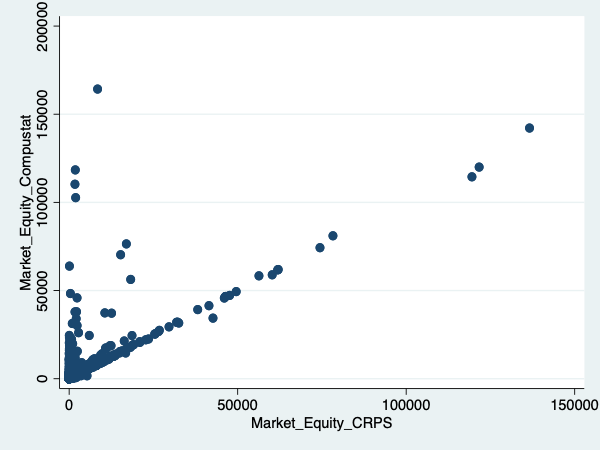
\includegraphics[scale=0.5]{m_equity_scatter}

\bigskip

\begin{tabular}{lc} \hline
 & (1) \\
VARIABLES & Market\_Equity\_Compustat \\ \hline
 &  \\
Market\_Equity\_CRPS & 1.050*** \\
 & (0.00701) \\
Constant & 108.4*** \\
 & (19.05) \\
 &  \\
Observations & 16,263 \\
 R-squared & 0.580 \\ \hline
\multicolumn{2}{c}{ Standard errors in parentheses} \\
\multicolumn{2}{c}{ *** p$<$0.01, ** p$<$0.05, * p$<$0.1} \\
\end{tabular}


\pagebreak

\section{Question 5}

Here, I compute the volatility of the return on assets.  First, I estimate the rolling standard deviation of the stock return over a 36 month window and then lever it up using market equity and total debt, as outlined in the problem set.

\begin{enumerate}

\item This is column (3) from panel A of my replication of table 2 (see question 2).

\item I find a much higher coefficient on initial book leverage, but I think mostly is due to the much lower sample due with observations getting lost in the merging process.  It would be interesting to try to improve the merge to get a more similar sample.  The coefficient on ROA volatility is very similar to that of cash-flow volatility, indicating that a one standard deviation change in these variables would have a similar effect on leverage.

\item This is column (6) from panel A of my replication of table 2 (see question 2).

\item Similar to (2).

\end{enumerate}

\bigskip

\begin{tabular}{lcc} \hline
 & (1) & (2) \\
VARIABLES & b\_lev\_tr & m\_lev\_tr \\ \hline
 &  &  \\
zee\_i\_b\_lev & 0.248*** &  \\
 & (0.00960) &  \\
zee\_l\_sales\_tr & 0.0203*** & 0.0336*** \\
 & (0.00173) & (0.00204) \\
zee\_m\_b\_tr & -0.0147*** & -0.0707*** \\
 & (0.00134) & (0.00165) \\
zee\_profit\_tr & -0.0342*** & -0.0544*** \\
 & (0.00147) & (0.00158) \\
zee\_tang\_tr & 0.0207*** & 0.0168*** \\
 & (0.00176) & (0.00201) \\
zee\_ind\_b\_lev & 0.0412*** & 0.0477*** \\
 & (0.00170) & (0.00176) \\
roa\_vol & -0.115*** & -0.154*** \\
 & (0.0126) & (0.0177) \\
pays\_dv & -0.0442*** & -0.0647*** \\
 & (0.00305) & (0.00362) \\
zee\_i\_m\_lev &  & 0.0864*** \\
 &  & (0.00238) \\
Constant & 0.284*** & 0.328*** \\
 & (0.00254) & (0.00306) \\
 &  &  \\
Observations & 56,970 & 51,313 \\
 R-squared & 0.370 & 0.492 \\ \hline
\multicolumn{3}{c}{ Robust standard errors in parentheses} \\
\multicolumn{3}{c}{ *** p$<$0.01, ** p$<$0.05, * p$<$0.1} \\
\end{tabular}


\end{document}

